\documentclass[12pt]{article}

%% Template for the semester

%% science symbols
\usepackage{amsmath}
\usepackage{amssymb}
\usepackage{amsthm}
\usepackage{bm}
\usepackage{cancel}
\usepackage{physics}
\usepackage{siunitx}
\usepackage{slashed}

%% general pretty stuff
\usepackage{float}
\usepackage{caption}
\usepackage{graphicx}
\usepackage{url}
\usepackage{enumitem}
\usepackage{hyperref}
\usepackage{tikz}
\usepackage{tikz-feynhand}

% setup options
\captionsetup{labelfont=bf}
\graphicspath{ {./figs/} }

% macros
\renewcommand{\L}{\mathcal{L}}
\renewcommand{\H}{\mathcal{H}}
\renewcommand{\l}{\ell}
\newcommand{\M}{\mathcal{M}}
\newcommand{\mcV}{\mathcal{V}}
\newcommand{\D}{\partial}
\newcommand{\veps}{\varepsilon}
\newcommand{\circled}[1]{\tikz[baseline=(char.base)]{
    \node[shape=circle,draw,inner sep=2pt](char){#1};}}

% mdframed environments
\usepackage[framemethod=TikZ]{mdframed}
\mdfsetup{skipabove=\topskip,skipbelow=\topskip}
\mdfdefinestyle{defstyle}{%
  linewidth=1pt,
  frametitlerule=true,
  frametitlebackgroundcolor=gray!40,
  backgroundcolor=gray!20,
  innertopmargin=\topskip
}

\mdtheorem[style=defstyle]{definition}{Definition}
\mdtheorem[style=defstyle]{theorem}{Theorem}
\mdtheorem[style=defstyle]{problem}{Problem}

\newenvironment{thebook}
{\begin{mdframed}[style=defstyle,frametitle={From the Book}]}{\end{mdframed}}


\title{\vspace{-3em}PHYS 202a HW 7}
\date{\today}

% setups
\graphicspath{ {./figs/} }

\newcommand\ttpf[8]{
  \begin{tikzpicture}
    \begin{feynhand}
      % vertices
      \vertex (p11) at (-1,1) {$#1$};
      \vertex (p12) at (-1,-1) {$#2$};
      \vertex (p21) at (1,1) {$#3$};
      \vertex (p22) at (1,-1) {$#4$};
      \vertex (a) at (0,0);
      % particles
      \propag #5 (p11) to (a);
      \propag #6 (p12) to (a);
      \propag #7 (a) to (p21);
      \propag #8 (a) to (p22);
    \end{feynhand}
  \end{tikzpicture}}

\begin{document}
\maketitle

\section{Renormalization for two scalars}
\begin{problem}
  Repeat the one-loop renormalization procedure of section 7.1 for two scalar field $\phi_{1,2}$ with the same mass $m_1=m_2=m$ and a quartic interaction of the form
  \begin{align*}
    \mathcal{L}_I=-\frac{\lambda_1}{4 !} \phi_1^4-\frac{\lambda_2}{4 !} \phi_2^4-\frac{g}{4} \phi_1^2 \phi_2^2
  \end{align*}
  There are now three renormalized couplings $\lambda_{1,2}^{\text {ren }}, g^{\text {ren }}$. Considering all five 2-to-2 scattering processes $1+1 \rightarrow 1+1,2+2 \rightarrow 2+2,1+2 \rightarrow 1+2,1+1 \rightarrow 2+2,2+2 \rightarrow 1+1$, and using the symmetric renormalization point $s=t=u=0$, write the equivalent of $(7.15)$ and express the renormalized couplings in terms of the original ones (to quadratic order). Show that they have the following features:
  \begin{itemize}
  \item If $g=0$ then $g^{\text{ren}}=0$.
  \item If $\lambda_1=\lambda_2$ then
    $\lambda_1^{\text{ren}}=\lambda_2^ {\text{ren}}$.
  \item If $\lambda_1=\lambda_2=3 g$ then
    $\lambda_1^{\text{ren}}=\lambda_2^{\text{ren}}=3 g^{\text{ren}}$.
  \end{itemize}
  Give a qualitative explanation for each of these features.

  The above feature show that the renormalized couplings are constrained by properties of the original Lagrangian. Nonetheless, renormalization can generate new couplings not present in the original Lagrangian. For example, if $\lambda_1=0$, can it happen that $\lambda_1^{\text {ren }} \neq 0$? Can renormalization also introduce a quartic coupling of the form $\phi_1 \phi_2^3$ in this theory? Why or why not?
\end{problem}

\subsection{Equivalent of 7.15}
We need to find the equivalent of the following 
\begin{align*}
  \mathcal{M}=\lambda^{\text{ren}}_{\text{sym}}
  \qty[1-\frac{\lambda^{\text{ren}}_{\text{sym}}}
  2\qty(\Delta I(s)+\Delta I(t)+\Delta I(u))]
\end{align*}
For the interaction Lagrangian above.

For the various tree-level processes the couplings are:
\begin{gather*}
  \mathcal{M}^{tree}(\phi_1\phi_1\to\phi_1\phi_1)=\lambda_1\\
  \mathcal{M}^{tree}(\phi_2\phi_2\to\phi_2\phi_2)=\lambda_2\\
  \mathcal{M}^{tree}(\phi_1\phi_2\to\phi_1\phi_2)=g\\
  \mathcal{M}^{tree}(\phi_1\phi_1\to\phi_2\phi_2)=g\\
  \mathcal{M}^{tree}(\phi_2\phi_2\to\phi_1\phi_1)=g
\end{gather*}
Since the only diagrams that contribute for each is:
\begin{figure}[H]
  \centering
  \ttpf{1}{1}{1}{1}{[sca]}{[sca]}{[sca]}{[sca]}
  \ttpf{2}{2}{2}{2}{}{}{}{}
  \ttpf{1}{2}{1}{2}{[sca]}{}{[sca]}{}
  \ttpf{1}{1}{2}{2}{[sca]}{[sca]}{}{}
  \ttpf{2}{2}{1}{1}{}{}{[sca]}{[sca]}
  \caption{Tree Level Diagrams}
\end{figure}
Note that the convention we have taken is that a dashed line represents a particle of type $1$ and a solid line represents a particle of type $2$

We then introduce the one-loop level diagrams, they each will be the $s,t,u$ channel-like diagrams from the $\phi^4$ theory, but with different particles dependening on the process.
\begin{itemize}
\item $1+1\to 1+1$
  \begin{figure}[H]
    \centering
    \begin{tikzpicture}
      \begin{feynhand}
        % vertices
        \vertex (p11) at (-1,1) {1}; \vertex (p12) at (-1,-1) {1};
        \vertex (p21) at (3,1) {1};  \vertex (p22) at (3,-1) {1};
        \vertex (a) at (0,0); \vertex (b) at (2,0);
        % particles
        \propag [sca] (p11) to (a); \propag [sca] (p12) to (a);
        \propag [sca] (b) to (p21); \propag [sca] (b) to (p22);
        % loop
        \propag [sca] (a) to [in=135, out=045, looseness=1.5] (b);
        \propag [sca] (b) to [out=225, in=315, looseness=1.5] (a);
      \end{feynhand}
    \end{tikzpicture}
    \begin{tikzpicture}
      \begin{feynhand}
        % vertices
        \vertex (p11) at (-1,1) {1}; \vertex (p12) at (-1,-1) {1};
        \vertex (p21) at (3,1) {1};  \vertex (p22) at (3,-1) {1};
        \vertex (a) at (0,0); \vertex (b) at (2,0);
        % particles
        \propag [sca] (p11) to (a); \propag [sca] (p12) to (a);
        \propag [sca] (b) to (p21); \propag [sca] (b) to (p22);
        % loop
        \propag (a) to [in=135, out=045, looseness=1.5] (b);
        \propag (b) to [out=225, in=315, looseness=1.5] (a);
      \end{feynhand}
    \end{tikzpicture}
    \\
    \begin{tikzpicture}
      \begin{feynhand}
        % vertices
        \vertex (p11) at (1.5,0) {1}; \vertex (p21) at (1.5,1.5) {1};
        \vertex (p12) at (-1.5,0) {1}; \vertex (p22) at (-1.5,1.5) {1};
        \vertex (a) at (0,0); \vertex (b) at (0,1.5);
        % particles
        \propag [sca] (p11) to (a); \propag [sca] (p12) to (a);
        \propag [sca] (b) to (p21); \propag [sca] (b) to (p22);
        % loop
        \propag [sca] (a) to [in=315, out=45, looseness=1] (b);
        \propag [sca] (b) to [out=225, in=125, looseness=1] (a);
      \end{feynhand}
    \end{tikzpicture}
    \begin{tikzpicture}
      \begin{feynhand}
        % vertices
        \vertex (p11) at (1.5,0) {1}; \vertex (p21) at (1.5,1.5) {1};
        \vertex (p12) at (-1.5,0) {1}; \vertex (p22) at (-1.5,1.5) {1};
        \vertex (a) at (0,0); \vertex (b) at (0,1.5);
        % particles
        \propag [sca] (p11) to (a); \propag [sca] (p12) to (a);
        \propag [sca] (b) to (p21); \propag [sca] (b) to (p22);
        % loop
        \propag (a) to [in=315, out=45, looseness=1] (b);
        \propag (b) to [out=225, in=125, looseness=1] (a);
      \end{feynhand}
    \end{tikzpicture}
    \begin{tikzpicture}
      \begin{feynhand}
        % vertices
        \vertex (p11) at (1.5,0) {1}; \vertex (p21) at (1.5,1.5) {1};
        \vertex (p12) at (-1.5,0) {1}; \vertex (p22) at (-1.5,1.5) {1};
        \vertex (a) at (0,0); \vertex (b) at (0,1.5);
        % particles
        \propag [sca] (p21) to (a);
        \propag [sca] (p12) to (a);
        \propag [sca] (b) to (p11);
        \propag [sca] (b) to (p22);
        % loop
        \propag [sca] (a) to [in=315, out=45, looseness=1] (b);
        \propag [sca] (b) to [out=225, in=125, looseness=1] (a);
      \end{feynhand}
    \end{tikzpicture}
    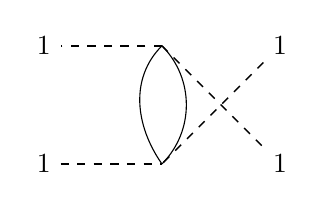
\begin{tikzpicture}
      \begin{feynhand}
        % vertices
        \vertex (p11) at (1.5,0) {1}; \vertex (p21) at (1.5,1.5) {1};
        \vertex (p12) at (-1.5,0) {1}; \vertex (p22) at (-1.5,1.5) {1};
        \vertex (a) at (0,0); \vertex (b) at (0,1.5);
        % particles
        \propag [sca] (p21) to (a);
        \propag [sca] (p12) to (a);
        \propag [sca] (b) to (p11);
        \propag [sca] (b) to (p22);
        % loop
        \propag (a) to [in=315, out=45, looseness=1] (b);
        \propag (b) to [out=225, in=125, looseness=1] (a);
      \end{feynhand}
    \end{tikzpicture}
    \caption{One-Loop Diagrams for $1+1\to1+1$}
  \end{figure}
  All of the diagrams with dotted loops are the same as the $\phi^4$ theory, so we have:
  \begin{align*}
    \mathcal{M}^{loop}_{\phi_1}=-\frac{\lambda_1^2}2\qty(I(s)+I(t)+I(u))
  \end{align*}
  The other three diagrams couple via the $g$ term:
  \begin{align*}
    \mathcal{M}^{loop}_{\phi_2}=-\frac{g^2}2\qty(I(s)+I(t)+I(u))
  \end{align*}
  So the overall matrix element at this level is given by:
  \begin{align*}
    \mathcal{M}^{1\ loop}(1+1\to1+1)=
    \lambda_1\qty(1-\frac{\lambda_1}2\qty(I(s)+I(t)+I(u)))
    -\frac{g^2}2\qty(I(s)+I(t)+I(u))
  \end{align*}
\item $2+2\to2+2$
  \begin{figure}[H]
    \centering
    \begin{tikzpicture}
      \begin{feynhand}
        % vertices
        \vertex (p11) at (-1,1) {2}; \vertex (p12) at (-1,-1) {2};
        \vertex (p21) at (3,1) {2};  \vertex (p22) at (3,-1) {2};
        \vertex (a) at (0,0); \vertex (b) at (2,0);
        % particles
        \propag (p11) to (a); \propag (p12) to (a);
        \propag (b) to (p21); \propag (b) to (p22);
        % loop
        \propag [sca] (a) to [in=135, out=045, looseness=1.5] (b);
        \propag [sca] (b) to [out=225, in=315, looseness=1.5] (a);
      \end{feynhand}
    \end{tikzpicture}
    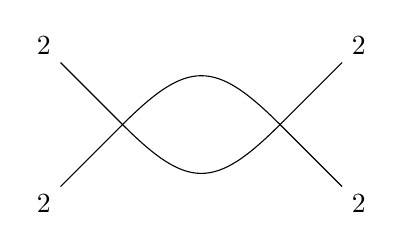
\begin{tikzpicture}
      \begin{feynhand}
        % vertices
        \vertex (p11) at (-1,1) {2}; \vertex (p12) at (-1,-1) {2};
        \vertex (p21) at (3,1) {2};  \vertex (p22) at (3,-1) {2};
        \vertex (a) at (0,0); \vertex (b) at (2,0);
        % particles
        \propag (p11) to (a); \propag (p12) to (a);
        \propag (b) to (p21); \propag (b) to (p22);
        % loop
        \propag (a) to [in=135, out=045, looseness=1.5] (b);
        \propag (b) to [out=225, in=315, looseness=1.5] (a);
      \end{feynhand}
    \end{tikzpicture}
    \\
    \begin{tikzpicture}
      \begin{feynhand}
        % vertices
        \vertex (p11) at (1.5,0) {2}; \vertex (p21) at (1.5,1.5) {2};
        \vertex (p12) at (-1.5,0) {2}; \vertex (p22) at (-1.5,1.5) {2};
        \vertex (a) at (0,0); \vertex (b) at (0,1.5);
        % particles
        \propag (p11) to (a); \propag (p12) to (a);
        \propag (b) to (p21); \propag (b) to (p22);
        % loop
        \propag [sca] (a) to [in=315, out=45, looseness=1] (b);
        \propag [sca] (b) to [out=225, in=125, looseness=1] (a);
      \end{feynhand}
    \end{tikzpicture}
    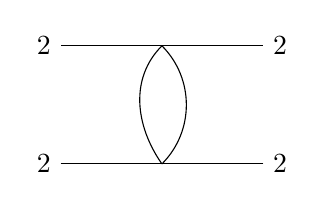
\begin{tikzpicture}
      \begin{feynhand}
        % vertices
        \vertex (p11) at (1.5,0) {2}; \vertex (p21) at (1.5,1.5) {2};
        \vertex (p12) at (-1.5,0) {2}; \vertex (p22) at (-1.5,1.5) {2};
        \vertex (a) at (0,0); \vertex (b) at (0,1.5);
        % particles
        \propag (p11) to (a); \propag (p12) to (a);
        \propag (b) to (p21); \propag (b) to (p22);
        % loop
        \propag (a) to [in=315, out=45, looseness=1] (b);
        \propag (b) to [out=225, in=125, looseness=1] (a);
      \end{feynhand}
    \end{tikzpicture}
    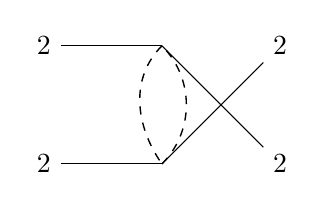
\begin{tikzpicture}
      \begin{feynhand}
        % vertices
        \vertex (p11) at (1.5,0) {2}; \vertex (p21) at (1.5,1.5) {2};
        \vertex (p12) at (-1.5,0) {2}; \vertex (p22) at (-1.5,1.5) {2};
        \vertex (a) at (0,0); \vertex (b) at (0,1.5);
        % particles
        \propag (p21) to (a);
        \propag (p12) to (a);
        \propag (b) to (p11);
        \propag (b) to (p22);
        % loop
        \propag [sca] (a) to [in=315, out=45, looseness=1] (b);
        \propag [sca] (b) to [out=225, in=125, looseness=1] (a);
      \end{feynhand}
    \end{tikzpicture}
    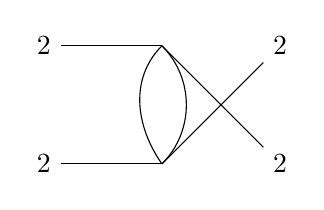
\begin{tikzpicture}
      \begin{feynhand}
        % vertices
        \vertex (p11) at (1.5,0) {2}; \vertex (p21) at (1.5,1.5) {2};
        \vertex (p12) at (-1.5,0) {2}; \vertex (p22) at (-1.5,1.5) {2};
        \vertex (a) at (0,0); \vertex (b) at (0,1.5);
        % particles
        \propag (p21) to (a);
        \propag (p12) to (a);
        \propag (b) to (p11);
        \propag (b) to (p22);
        % loop
        \propag (a) to [in=315, out=45, looseness=1] (b);
        \propag (b) to [out=225, in=125, looseness=1] (a);
      \end{feynhand}
    \end{tikzpicture}
    \caption{One-Loop Diagrams for $2+2\to2+2$}
  \end{figure}
  Only the coupling constant changed. So the matrix element is:
  \begin{align*}
    \mathcal{M}^{1\ loop}(2+2\to2+2)=
    \lambda_2\qty(1-\frac{\lambda_2}2\qty(I(s)+I(t)+I(u)))
    -\frac{g^2}2\qty(I(s)+I(t)+I(u))
  \end{align*}
\item $1+2\to1+2$
  \begin{figure}[H]
    \centering
    \begin{tikzpicture}
      \begin{feynhand}
        % vertices
        \vertex (p11) at (-1,1) {1}; \vertex (p12) at (-1,-1) {2};
        \vertex (p21) at (3,1) {1};  \vertex (p22) at (3,-1) {2};
        \vertex (a) at (0,0); \vertex (b) at (2,0);
        % particles
        \propag [sca] (p11) to (a); \propag (p12) to (a);
        \propag [sca] (b) to (p21); \propag (b) to (p22);
        % loop
        \propag (a) to [in=135, out=045, looseness=1.5] (b);
        \propag [sca] (b) to [out=225, in=315, looseness=1.5] (a);
      \end{feynhand}
    \end{tikzpicture}
    \\
    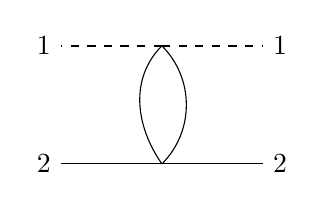
\begin{tikzpicture}
      \begin{feynhand}
        % vertices
        \vertex (p11) at (1.5,0) {2}; \vertex (p21) at (1.5,1.5) {1};
        \vertex (p12) at (-1.5,0) {2}; \vertex (p22) at (-1.5,1.5) {1};
        \vertex (a) at (0,0); \vertex (b) at (0,1.5);
        % particles
        \propag (p11) to (a); \propag (p12) to (a);
        \propag [sca] (b) to (p21); \propag [sca] (b) to (p22);
        % loop
        \propag (a) to [in=315, out=45, looseness=1] (b);
        \propag (b) to [out=225, in=125, looseness=1] (a);
      \end{feynhand}
    \end{tikzpicture}
    \begin{tikzpicture}
      \begin{feynhand}
        % vertices
        \vertex (p11) at (1.5,0) {2}; \vertex (p21) at (1.5,1.5) {1};
        \vertex (p12) at (-1.5,0) {2}; \vertex (p22) at (-1.5,1.5) {1};
        \vertex (a) at (0,0); \vertex (b) at (0,1.5);
        % particles
        \propag (p11) to (a); \propag (p12) to (a);
        \propag [sca] (b) to (p21); \propag [sca] (b) to (p22);
        % loop
        \propag [sca] (a) to [in=315, out=45, looseness=1] (b);
        \propag [sca] (b) to [out=225, in=125, looseness=1] (a);
      \end{feynhand}
    \end{tikzpicture}
    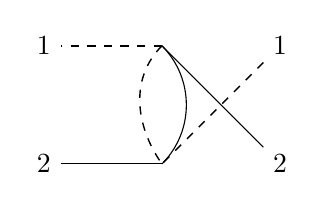
\begin{tikzpicture}
      \begin{feynhand}
        % vertices
        \vertex (p11) at (1.5,0) {2}; \vertex (p21) at (1.5,1.5) {1};
        \vertex (p12) at (-1.5,0) {2}; \vertex (p22) at (-1.5,1.5) {1};
        \vertex (a) at (0,0); \vertex (b) at (0,1.5);
        % particles
        \propag [sca] (p21) to (a);
        \propag (p12) to (a);
        \propag (b) to (p11);
        \propag [sca] (b) to (p22);
        % loop
        \propag (a) to [in=315, out=45, looseness=1] (b);
        \propag [sca] (b) to [out=225, in=125, looseness=1] (a);
      \end{feynhand}
    \end{tikzpicture}
    \caption{One-Loop Diagrams for $1+2\to1+2$}
  \end{figure}
  The Matrix element is
  \begin{align*}
    \mathcal{M}^{1\ loop}(1+2\to1+2)=
    g\qty(1-g\qty(I(s)+I(u))-\frac12\qty(\lambda_1+\lambda_2)I(t))
  \end{align*}
\item $1+1\to2+2$
  \begin{figure}[H]
    \centering
    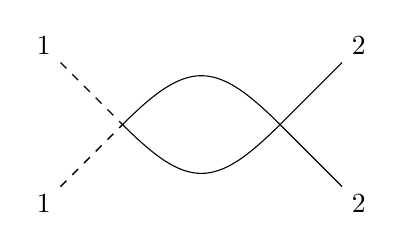
\begin{tikzpicture}
      \begin{feynhand}
        % vertices
        \vertex (p11) at (-1,1) {1}; \vertex (p12) at (-1,-1) {1};
        \vertex (p21) at (3,1) {2};  \vertex (p22) at (3,-1) {2};
        \vertex (a) at (0,0); \vertex (b) at (2,0);
        % particles
        \propag [sca] (p11) to (a); \propag [sca] (p12) to (a);
        \propag (b) to (p21); \propag (b) to (p22);
        % loop
        \propag (a) to [in=135, out=045, looseness=1.5] (b);
        \propag (b) to [out=225, in=315, looseness=1.5] (a);
      \end{feynhand}
    \end{tikzpicture}
    \begin{tikzpicture}
      \begin{feynhand}
        % vertices
        \vertex (p11) at (-1,1) {1}; \vertex (p12) at (-1,-1) {1};
        \vertex (p21) at (3,1) {2};  \vertex (p22) at (3,-1) {2};
        \vertex (a) at (0,0); \vertex (b) at (2,0);
        % particles
        \propag [sca] (p11) to (a); \propag [sca] (p12) to (a);
        \propag (b) to (p21); \propag (b) to (p22);
        % loop
        \propag [sca] (a) to [in=135, out=045, looseness=1.5] (b);
        \propag [sca] (b) to [out=225, in=315, looseness=1.5] (a);
      \end{feynhand}
    \end{tikzpicture}
    \\
    \begin{tikzpicture}
      \begin{feynhand}
        % vertices
        \vertex (p11) at (1.5,0) {2}; \vertex (p21) at (1.5,1.5) {2};
        \vertex (p12) at (-1.5,0) {1}; \vertex (p22) at (-1.5,1.5) {1};
        \vertex (a) at (0,0); \vertex (b) at (0,1.5);
        % particles
        \propag (p11) to (a);
        \propag [sca] (p12) to (a);
        \propag (b) to (p21);
        \propag [sca] (b) to (p22);
        % loop
        \propag [sca] (a) to [in=315, out=45, looseness=1] (b);
        \propag (b) to [out=225, in=125, looseness=1] (a);
      \end{feynhand}
    \end{tikzpicture}
    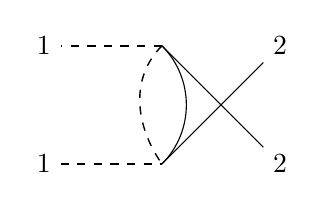
\begin{tikzpicture}
      \begin{feynhand}
        % vertices
        \vertex (p11) at (1.5,0) {2}; \vertex (p21) at (1.5,1.5) {2};
        \vertex (p12) at (-1.5,0) {1}; \vertex (p22) at (-1.5,1.5) {1};
        \vertex (a) at (0,0); \vertex (b) at (0,1.5);
        % particles
        \propag (p21) to (a);
        \propag [sca] (p12) to (a);
        \propag (b) to (p11);
        \propag [sca] (b) to (p22);
        % loop
        \propag (a) to [in=315, out=45, looseness=1] (b);
        \propag [sca] (b) to [out=225, in=125, looseness=1] (a);
      \end{feynhand}
    \end{tikzpicture}
    \caption{One-Loop Diagrams for $1+1\to2+2$}
  \end{figure}
  Matrix element:
  \begin{align*}
    \mathcal{M}^{1\ loop}(1+1\to2+2)=
    g\qty(1-g\qty(I(t)+I(u))-\frac12(\lambda_1+\lambda_2)I(s))
  \end{align*}
\item $2+2\to1+1$
  \begin{figure}[H]
    \centering
    \begin{tikzpicture}
      \begin{feynhand}
        % vertices
        \vertex (p22) at (-1,1) {2}; \vertex (p21) at (-1,-1) {2};
        \vertex (p12) at (3,1) {1}; \vertex (p11) at (3,-1) {1};
        \vertex (a) at (0,0); \vertex (b) at (2,0);
        % particles
        \propag [sca] (p11) to (b); \propag [sca] (p12) to (b);
        \propag (a) to (p21); \propag (a) to (p22);
        % loop
        \propag (a) to [in=135, out=045, looseness=1.5] (b);
        \propag (b) to [out=225, in=315, looseness=1.5] (a);
      \end{feynhand}
    \end{tikzpicture}
    \begin{tikzpicture}
      \begin{feynhand}
        % vertices
        \vertex (p22) at (-1,1) {2}; \vertex (p21) at (-1,-1) {2};
        \vertex (p12) at (3,1) {1}; \vertex (p11) at (3,-1) {1};
        \vertex (a) at (0,0); \vertex (b) at (2,0);
        % particles
        \propag [sca] (p11) to (b); \propag [sca] (p12) to (b);
        \propag (a) to (p21); \propag (a) to (p22);
        % loop
        \propag [sca] (a) to [in=135, out=045, looseness=1.5] (b);
        \propag [sca] (b) to [out=225, in=315, looseness=1.5] (a);
      \end{feynhand}
    \end{tikzpicture}
    \\
    \begin{tikzpicture}
      \begin{feynhand}
        % vertices
        \vertex (p11) at (1.5,0) {1}; \vertex (p21) at (1.5,1.5) {1};
        \vertex (p12) at (-1.5,0) {2}; \vertex (p22) at (-1.5,1.5) {2};
        \vertex (a) at (0,0); \vertex (b) at (0,1.5);
        % particles
        \propag [sca] (p11) to (a);
        \propag (p12) to (a);
        \propag [sca] (b) to (p21);
        \propag (b) to (p22);
        % loop
        \propag [sca] (a) to [in=315, out=45, looseness=1] (b);
        \propag (b) to [out=225, in=125, looseness=1] (a);
      \end{feynhand}
    \end{tikzpicture}
    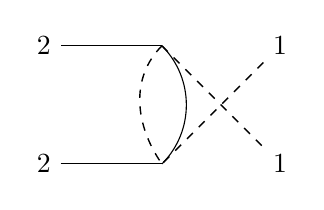
\begin{tikzpicture}
      \begin{feynhand}
        % vertices
        \vertex (p11) at (1.5,0) {1}; \vertex (p21) at (1.5,1.5) {1};
        \vertex (p12) at (-1.5,0) {2}; \vertex (p22) at (-1.5,1.5) {2};
        \vertex (a) at (0,0); \vertex (b) at (0,1.5);
        % particles
        \propag [sca](p21) to (a);
        \propag (p12) to (a);
        \propag [sca] (b) to (p11);
        \propag (b) to (p22);
        % loop
        \propag (a) to [in=315, out=45, looseness=1] (b);
        \propag [sca] (b) to [out=225, in=125, looseness=1] (a);
      \end{feynhand}
    \end{tikzpicture}
    \caption{One-Loop Diagrams for $2+2\to1+1$}
  \end{figure}
  Matrix Element:
  \begin{align*}
    \mathcal{M}^{1\ loop}(2+2\to1+1)=
    g\qty(1-g\qty(I(t)+I(u))-\frac12(\lambda_1+\lambda_2)I(s))
  \end{align*}
\end{itemize}
We want to renormalize about the symmetric point, $s=t=u=0$, at which the matrix elements look like:
\begin{gather*}
  \mathcal{M}^{11\to11}(0,0,0)=
  \lambda_1\qty(1-\frac{\lambda_1}23I(0))-\frac{g^2}23I(0)\\
  \mathcal{M}^{22\to22}(0,0,0)=
  \lambda_2\qty(1-\frac{\lambda_2}23I(0))-\frac{g^2}23I(0)\\
  \mathcal{M}^{12\to12}(0,0,0)=
  \mathcal{M}^{11\to22}(0,0,0)=
  \mathcal{M}^{11\to22}(0,0,0)=
  g\qty(1-2gI(0)-\frac12(\lambda_1+\lambda_2)I(0))
\end{gather*}
These each then define the renormalized coupling values:
\begin{align*}
  \lambda_1^{ren}=\lambda_1\qty(1-\frac{\lambda_1}23I(0))-\frac{g^2}23I(0)\\
  \lambda_2^{ren}=\lambda_2\qty(1-\frac{\lambda_2}23I(0))-\frac{g^2}23I(0)\\
  g^{ren}=g\qty(1-2gI(0)-\frac12(\lambda_1+\lambda_2)I(0))
\end{align*}
Here we heavily made use of Mathematica to perform series expansions.

The first terms to solve for are $\lambda_{1/2}$ in terms of $\lambda_{1/2}^{ren}$ and the bare coupling $g$:
\begin{align*}
  \lambda_{1/2}=\frac{1\pm\sqrt{1-6\lambda_{1/2}^{ren}I(0)-9g^2I(0)}}{3I(0)^2}
\end{align*}
Notice that there are 2 solutions, but we chose the one that plays better with the series expansion of $\sqrt{1+x}$:
\begin{align*}
  \sqrt{1+x}\approx1-\frac{x}{2}-\frac{x^2}{8}+\order{x^3}
\end{align*}
Series expand this in terms of $\lambda_{1/2}$ and $g$ up to quadratic order, which is the minus solution. This gives:
\begin{align*}
  \lambda_{1/2}\approx\lambda_{1/2}^{ren}+\frac32\lambda_{1/2}^{ren}I(0)
  +g^2\qty(\frac32I(0)+\frac92\lambda_{1/2}^{ren}(I(0))^2
  +\frac{81}4(\lambda_{1/2}^{ren})^2(I(0))^3)
\end{align*}
However, note that the second two terms are above second order, since they involve combinations like $g^2\lambda_{1/2}^{ren}$ and those terms are sufficiently small so that we can ignore them, to say:
\begin{align*}
  \lambda_{1/2}\approx\lambda_{1/2}^{ren}
  +\frac32\lambda_{1/2}^{ren}I(0)
  +\frac32g^2I(0)
\end{align*}
We can then use these to solve for $g$ in terms of all of the renormalized couplings. If we naively sub in what we had for each of $\lambda_1$ and $\lambda_2$, we see:
\begin{align*}
  g^{ren}=g\qty[1-2g I(0)-\frac12I(0)
  \qty(\lambda^{ren}_1+\lambda^{ren}_2
  +\frac32I(0)((\lambda_1^{ren})^2+(\lambda_2^{ren})^2)+3g^2I(0))]
\end{align*}
However we immediately notice that everything besides the first two terms in the parenthetical will be third order or higher, so we can ignore them, giving:
\begin{align*}
  g^{ren}=g\qty[1-2g I(0)-\frac{\lambda^{ren}_1+\lambda^{ren}_2}2I(0)]
\end{align*}
The solution of $g$ in terms of the renormalized couplings is:
\begin{align*}
  g=\frac{1-\frac12I(0)(\lambda_1^{ren}+\lambda_2^{ren})\pm
    \sqrt{-8g^{ren}I(0)+(-1+\frac12I(0)(\lambda_1^{ren}+\lambda_2^{ren}))^2}}
  {4I(0)}
\end{align*}
Using the power of Mathematica to expand this gives something gross, so we can just skip to the nice result to lowest order:
\begin{align*}
  g\approx g^{ren}\qty(1+2g^{ren}I(0)+
  \frac{\lambda_1^{ren}+\lambda_2^{ren}}2I(0))
\end{align*}
Note that even though we have $\lambda_{1/2}^{ren}$ in terms of $g$, since to lowest order (which is all we can insert in terms of $g^2$) $g=g^{ren}$, and we can then finally have the bare couplings in terms of the renormalized ones:
\begin{align*}
  \lambda_{1/2}&=\lambda_{1/2}^{ren}\qty(1+\frac32\lambda_{1/2}^{ren}I(0))
  +\frac32(g^{ren})^2I(0)\\
  g&=g^{ren}\qty(1+2g^{ren}I(0)+\frac{\lambda_1^{ren}+\lambda_2^{ren}}2I(0))
\end{align*}
Note the structure of these lead to the exact same conversion of the Matrix elements, where we have a coupling turns into its renormalized equivalent, and an integral has a negative $I(0)$ associated with it, so our matrix elements become:
\begin{equation}
  \boxed{
    \begin{aligned}
      \mathcal{M}^{11\to11}&=\lambda_1^{ren}
      -\frac12\qty((\lambda_1^{ren})^2+(g^{ren})^2)
      (\Delta I(s)+\Delta I(t)+\Delta I(u))\\
      \mathcal{M}^{22\to22}&=\lambda_2^{ren}
      -\frac12\qty((\lambda_2^{ren})^2+(g^{ren})^2)
      (\Delta I(s)+\Delta I(t)+\Delta I(u))\\
      \mathcal{M}^{12\to12}&=
      g^{ren}\qty(1-g^{ren}(\Delta I(s)+\Delta I(u))
      -\frac{\lambda_1^{ren}+\lambda_2^{ren}}2\Delta I(t))\\
      \mathcal{M}^{11\to22}&=
      g^{ren}\qty(1-g^{ren}(\Delta I(t)+\Delta I(u))
      -\frac{\lambda_1^{ren}+\lambda_2^{ren}}2\Delta I(s))\\
      \mathcal{M}^{22\to11}&=
      g^{ren}\qty(1-g^{ren}(\Delta I(t)+\Delta I(u))
      -\frac{\lambda_1^{ren}+\lambda_2^{ren}}2\Delta I(s))
    \end{aligned}}
\end{equation}
Which is the equivalent of 7.15

\subsection{Features of the Couplings}
The renormalized couplings in terms of the bare couplings are given by:
\begin{equation}
  \boxed{\begin{gathered}
    \lambda_1^{ren}=\lambda_1\qty(1-\frac{\lambda_1}23I(0))-\frac{g^2}23I(0)\\
    \lambda_2^{ren}=\lambda_2\qty(1-\frac{\lambda_2}23I(0))-\frac{g^2}23I(0)\\
    g^{ren}=g\qty(1-2gI(0)-\frac12(\lambda_1+\lambda_2)I(0))
  \end{gathered}}
\end{equation}
First note that $g^{ren}$ is proportional to the bare coupling, so that way if the bare coupling is $0$, so is $g^{ren}$. Hence:
\begin{align*}
  g=0\implies g^{ren}=0
\end{align*}
Qualitatively, this means that there is no way to renormalize 2 uncoupled theories to make them coupled. Without the $g$ term, the interaction term we initially studied has no mixing between $\phi_1$ and $\phi_2$ fields, so this feature tells us that there is no way to make 2 independent fields interact through renormalization.

For the second feature, note what happens if we subtract the equations for $\lambda_2^{ren}$ from the equation for $\lambda_1^{ren}$:
\begin{align*}
  \lambda_1^{ren}-\lambda_2^{ren}=\qty(\lambda_1-\lambda_2)
  \qty(1-\frac32I(0)(\lambda_1+\lambda_2))
\end{align*}
Then, if $\lambda_1=\lambda_2$, we have $\lambda_1-\lambda_2=0$, which means:
\begin{align*}
  \lambda_1^{ren}-\lambda_2^{ren}=0
\end{align*}
Hence we get:
\begin{align*}
  \lambda_1=\lambda_2\implies\lambda_1^{ren}=\lambda_2^{ren}
\end{align*}
If the two couplings are equal, then there is essentially no difference between a $\phi_1$ particle and a $\phi_2$ particle, we could almost completely factor the Lagrangian into terms acting on $\phi_1+\phi_2$. To me this denotes some sort of symmetry between the $\phi_1$ and $\phi_2$ particles. This can be seen in the interaction Lagrangian if we set $\lambda_1=\lambda_2=\lambda$, we would have:
\begin{align*}
  \L_I=\frac{\lambda}{4!}\qty(\phi_1^4+\phi_2^4)+\frac{g}4\phi_1^2\phi_2^2
\end{align*}
So there is no difference between a $\phi_1$ and $\phi_2$

We can clearly see this even at the diagram level, since the diagrams for $1+1\to2+2$ is given in terms of $2+2\to1+1$ by swapping 1s with 2s and vice versa, this can be done with any process.

The next property is easiest to see if we define a term $\lambda$ to encompass all of the terms, we choose:
\begin{gather*}
  \lambda_1=\lambda_2=\lambda \\g=\frac\lambda3
\end{gather*}
Plugging these into the equations for the couplings we have:
\begin{align*}
  \lambda_1^{ren}&=\lambda\qty(1-\frac32\lambda I(0))-\frac16\lambda^2I(0)
  =\lambda\qty(1-\frac53\lambda I(0))\\
  \lambda_2^{ren}&=\lambda\qty(1-\frac32\lambda I(0))-\frac16\lambda^2I(0)
  =\lambda\qty(1-\frac53\lambda I(0))\\
  3g^{ren}&=\lambda\qty(1-\frac53\lambda I(0))
\end{align*}
Hence we explicitly have:
\begin{align*}
  \lambda_1=\lambda_2=3g\implies
  \lambda_1^{ren}=\lambda_2^{ren}=3g^{ren}
\end{align*}
This extends the symmetry between $\phi_1$ and $\phi_2$ to their cross terms as well. We can explicitly count at tree level there is 1 $\lambda_1$ vertex, 1 $\lambda_2$ vertex, and 3 $g$ vertices. At 1-loop, you can count above that this ratio remains the same, with 10 $\lambda_1$ and $\lambda_2$ vertices, and 30 $g$ vertices.

This symmetry makes the Lagrangian almost look like it can be factored into terms acting only on the quantity $(\phi_1+\phi_2)$, making it seem like there is no difference whatsoever to these fields, and is simply a expansion of a much simpler field

\subsection{New Couplings}
From the explicit calculation we did before, if $\lambda_1=0$, we have:
\begin{align*}
  \lambda_1^{ren}=-\frac32g^2I(0)
\end{align*}
So there can be a renormalization induced $\lambda_1$ term.

However, in order to induce a term like $\phi_1\phi_2^3$, we would need something like the following vertex:
\begin{figure}[H]
  \centering
  \ttpf{1}{2}{2}{2}{[sca]}{}{}{}
  \caption{Hypothetical Vertex}
  \label{fig:1}
\end{figure}
However, no counterterm that would be introduced by renormalization would look like $\phi_1\phi_2^3$, and the vertex in Figure~\ref{fig:1} simply does not exist in the Lagrangian, and the counterterm Lagrangian only has terms that are in the original Lagrangian.
\newpage
\section{Counterterms}
\begin{problem}
  Consider a scalar field with a cubic self-interaction:
  \begin{align*}
    \mathcal{L}=\frac{1}{2} \partial_\mu \phi \partial^\mu \phi-\frac{m^2}{2} \phi^2-\frac{\lambda}{3 !} \phi^3
  \end{align*}
  Compute the one-loop counterterms, as a function of the physical mass $m$ and the physical coupling $\lambda$, in dimensional regularization, for the mass and the wave function of $\phi$.
\end{problem}
\end{document}